\chapter{Mission Modeling Workflow and Selected Code}
\label{appendix:framework-workflow}

This representative workflow illustrates the second objective through mission construction, requirement management, linked analyses and verification.
The engineer iterates until satisfied with the assessment, saves the mission as a Python file and commits it with the decision rationale as the Git commit message.
The synthetic example demonstrates selected passing checks while retaining unresolved mission requirements.

\begin{figure}[!htbp]
\centering
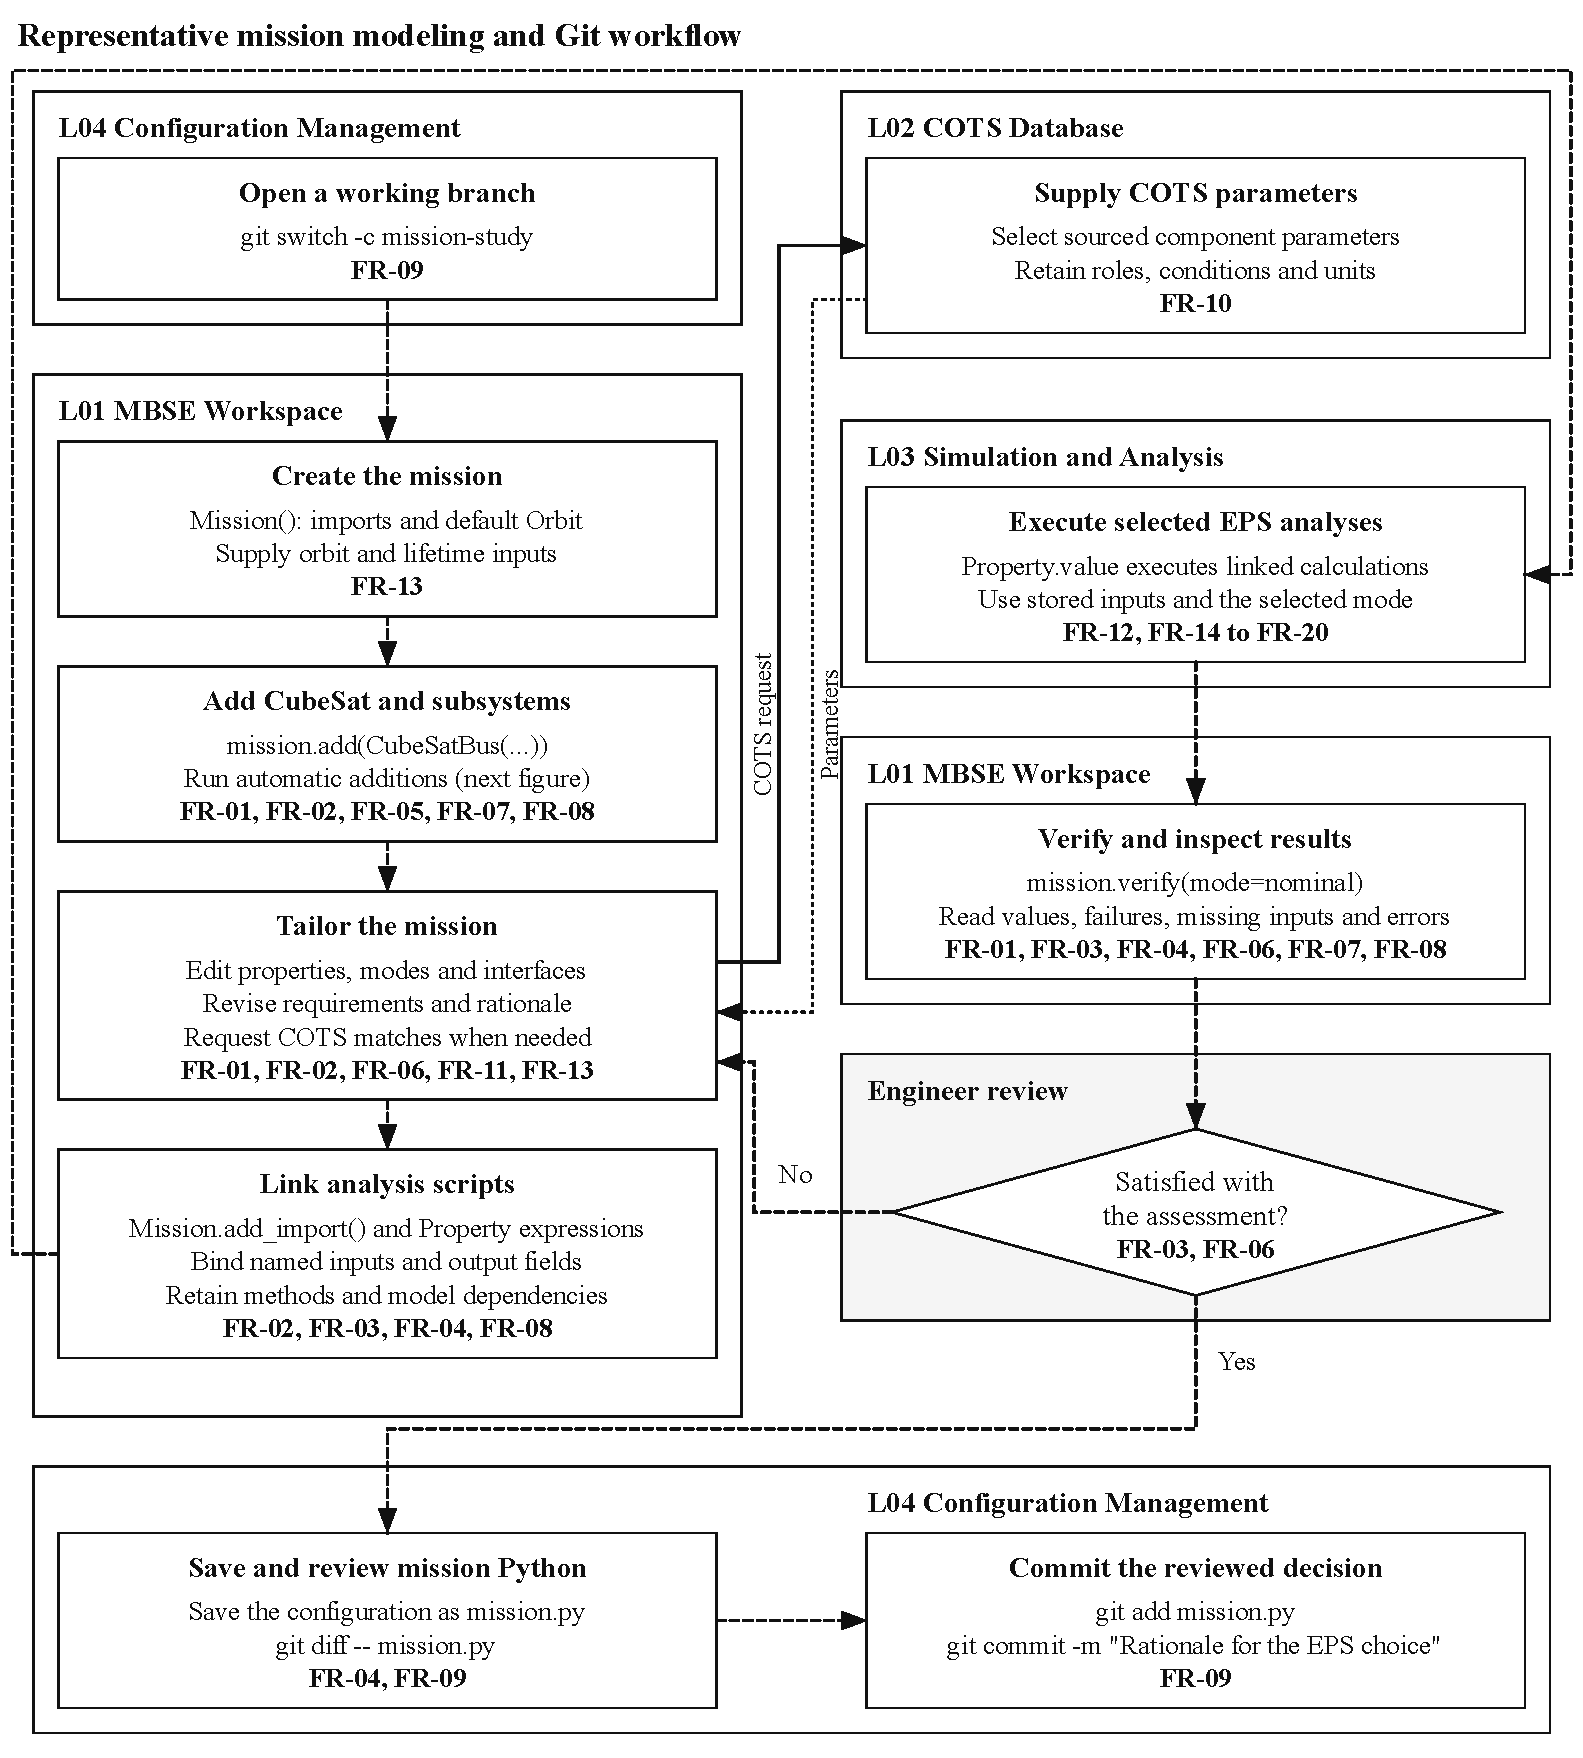
\includegraphics[width=0.94\linewidth]{fig/model-appendices/mission-workflow.pdf}
\caption[Representative mission modeling and Git workflow.]{A representative use of the Python models, also exposed through the GUI. Dashed arrows show control flow. The return path revises the mission, its inputs or its requirements before executing the stored analyses again. Satisfaction is an engineering review decision that includes assessment coverage and assumptions. The Git operations are performed by the engineer after saving the mission, and the commit message records the rationale for the accepted configuration.}
\label{fig:mission-modeling-workflow}
\end{figure}
\clearpage

\begin{figure}[p]
\centering
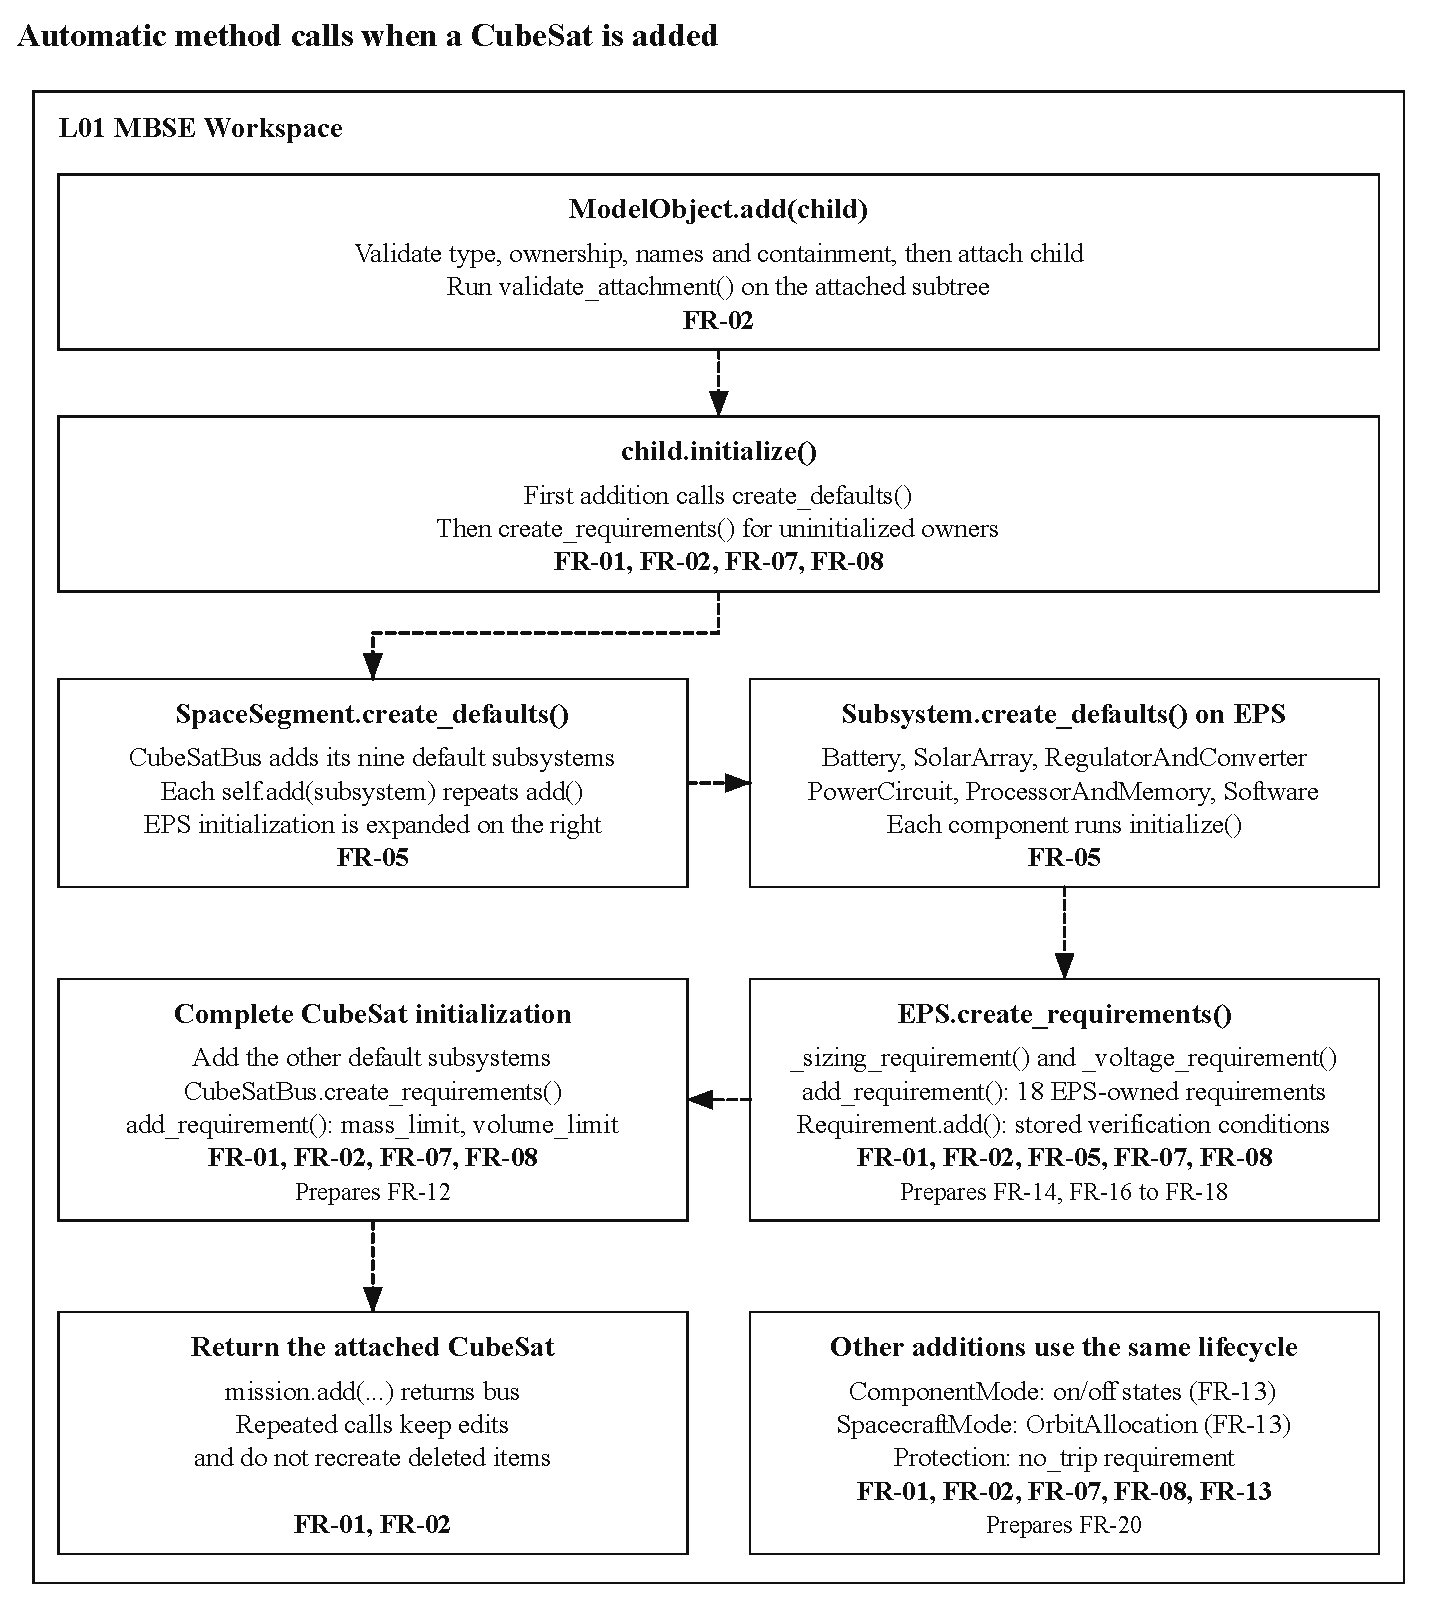
\includegraphics[width=\linewidth]{fig/model-appendices/addition-lifecycle.pdf}
\caption[Method calls and automatic additions during mission construction.]{Expansion of the CubeSat addition in Figure~\ref{fig:mission-modeling-workflow}. Dashed arrows show the successful first-addition path through the shared add() and initialize() methods. Nested additions use the same methods. EPS initialization adds four numerical component defaults and 18 EPS-owned requirements. CubeSat initialization also creates the mass and volume requirements. The lower right box identifies the hooks used by other illustrated additions. An attachment error removes the newly attached child and newly generated requirements. Restoration can suppress initialization, and initialization flags preserve subsequent edits and deliberate deletions.}
\label{fig:mission-addition-lifecycle}
\end{figure}
\clearpage

\begin{figure}[p]
\centering
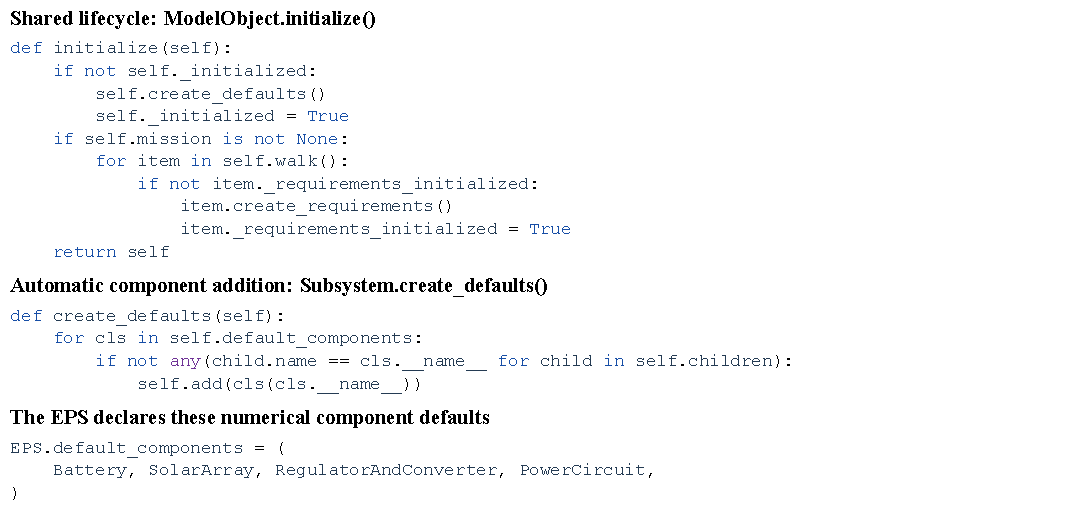
\includegraphics[width=\linewidth]{fig/model-appendices/initialization-code.pdf}
\caption[Source excerpts for initialization and default component creation.]{The shared initialization method creates defaults once and assigns requirements after their owners join a mission. The subsystem method adds its declared component classes through the same add() lifecycle. The final excerpt identifies the four numerical EPS defaults expanded in Figure~\ref{fig:mission-addition-lifecycle}. The complete source is in Appendix~\ref{appendix:framework-code}.}
\label{fig:mission-initialization-code}
\end{figure}

\begin{figure}[p]
\centering
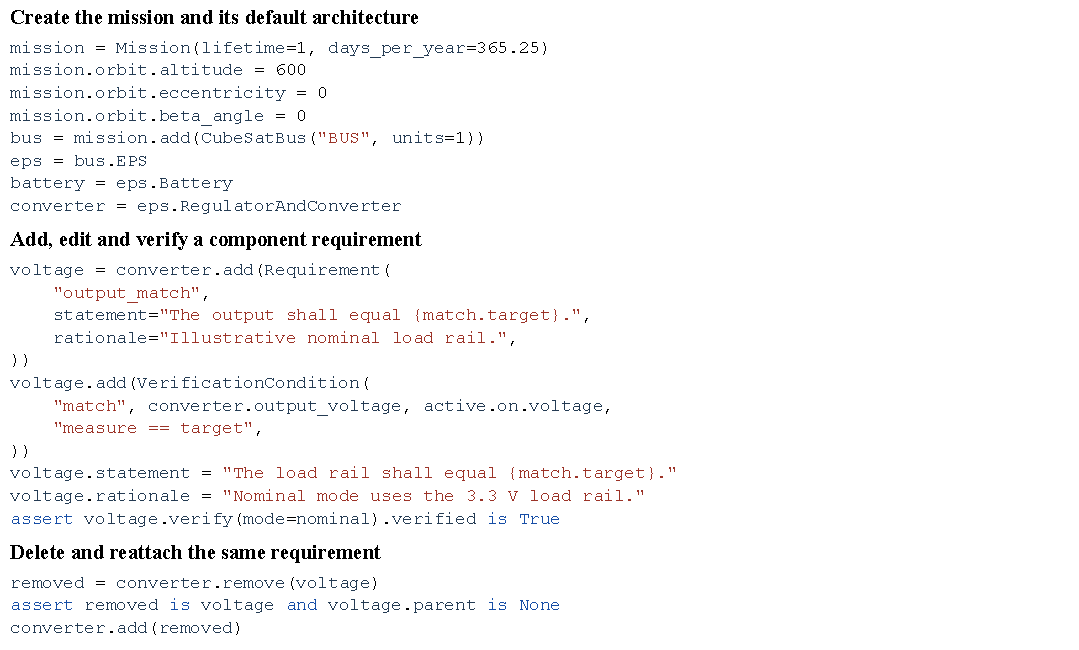
\includegraphics[width=\linewidth]{fig/model-appendices/mission-and-requirements.pdf}
\caption[Mission construction and requirement operations.]{Selected executable Python calls construct a mission and add an owned converter requirement with a verification condition. The mode, state and interface definitions are shown in Figures~\ref{fig:eps-modes-states} and~\ref{fig:eps-property-interfaces}. Updating its statement and rationale retains the condition's links to the converter output and load state. verify() evaluates the stored condition for the selected nominal mode. remove() detaches the requirement and excludes it from mission verification, and add() can reattach the same object. These calls illustrate adding, editing, updating, verifying and deleting requirements without reproducing the full source appendix.}
\label{fig:mission-requirement-operations}
\end{figure}
\clearpage

\begin{figure}[p]
\centering
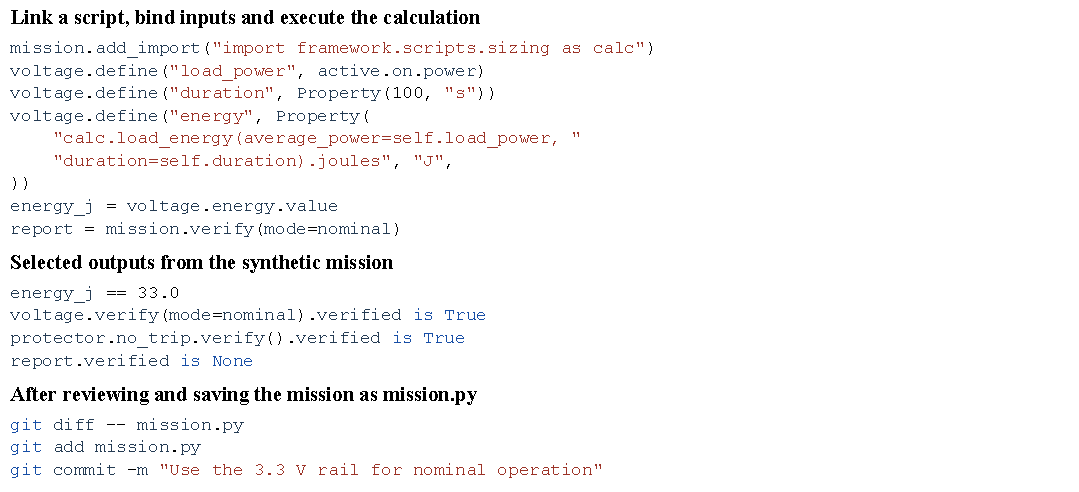
\includegraphics[width=\linewidth]{fig/model-appendices/scripts-and-commit.pdf}
\caption[Linking analyses, executing verification and recording rationale.]{An explicit import makes a calculation available to property expressions. Named Property inputs bind 0.33~W and 100~s to the load energy function, and the selected output evaluates to 33~J when energy.value is read. mission.verify() executes the stored verification conditions and their dependencies in the selected mode. The two illustrated requirements pass, while the complete mission result remains unresolved because other inputs are unset. After reviewing and saving the configuration, the engineer stages its Python file and commits it with a rationale message. The Git commands are illustrative and were not executed to create this report.}
\label{fig:mission-scripts-commit}
\end{figure}
\clearpage
